% Source: src-b19b233abb266d1b051ded3c332a399c1722d8192d07ce1bf2234dda57bd25bc, PDF p.1.
% Topology follows the source; oblique projection is schematic, not metric.
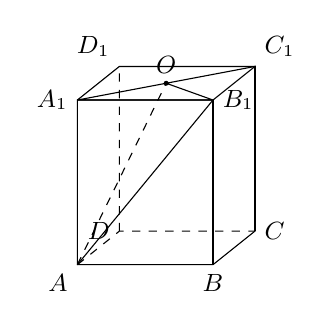
\begin{tikzpicture}[scale=0.82, every node/.style={font=\small}]
  \coordinate (A) at (0,0);
  \coordinate (B) at (2.1,0);
  \coordinate (C) at (2.75,0.52);
  \coordinate (D) at (0.65,0.52);
  \coordinate (A1) at (0,2.55);
  \coordinate (B1) at (2.1,2.55);
  \coordinate (C1) at (2.75,3.07);
  \coordinate (D1) at (0.65,3.07);
  \coordinate (O) at (1.375,2.81);
  \draw (A)--(B)--(C)--(C1)--(B1)--(A1)--cycle;
  \draw (C1)--(D1)--(A1);
  \draw[dashed] (A)--(D)--(C) (D)--(D1);
  \draw (A)--(A1) (B)--(B1) (C)--(C1);
  \draw (A1)--(C1) (A1)--(B1) (O)--(B1) (A)--(B1);
  \draw[dashed] (A)--(O);
  \fill (O) circle (1.1pt);
  \node[below left] at (A) {$A$};
  \node[below] at (B) {$B$};
  \node[right] at (C) {$C$};
  \node[left] at (D) {$D$};
  \node[left] at (A1) {$A_1$};
  \node[right] at (B1) {$B_1$};
  \node[above right] at (C1) {$C_1$};
  \node[above left] at (D1) {$D_1$};
  \node[above] at (O) {$O$};
\end{tikzpicture}
